% problem.tex -- a self-contained motivated-example figure.
\documentclass[tikz,border=3pt]{standalone}
\usepackage[dvipsnames]{xcolor}
\usetikzlibrary{arrows.meta,positioning,fit,shapes.geometric}
\newcommand{\VIS}{\mathsf{VIS}}
\newcommand{\AR}{\mathsf{AR}}
\newcommand{\ser}{\mathsf{SER}}
\newcommand{\si}{\mathsf{SI}}
\newcommand{\WR}{\mathsf{WR}}
\newcommand{\WW}{\mathsf{WW}}
\newcommand{\RW}{\mathsf{RW}}
\begin{document}
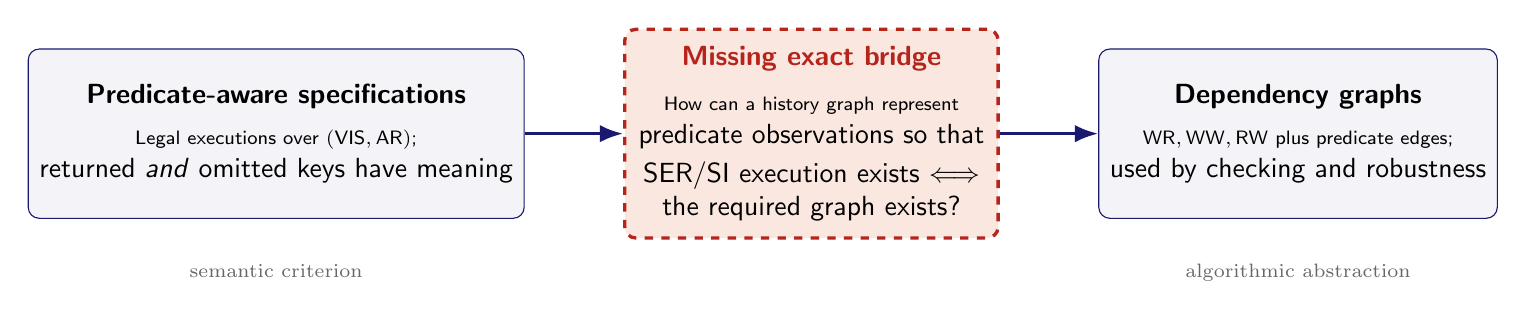
\begin{tikzpicture}[
  >=Latex, font=\sffamily,
  card/.style={draw=MidnightBlue,rounded corners=4pt,fill=MidnightBlue!5,
    minimum width=4.3cm,minimum height=2.15cm,align=center,inner sep=4pt},
  gap/.style={draw=BrickRed,rounded corners=4pt,dashed,very thick,
    fill=BrickRed!8,minimum width=4.1cm,minimum height=2.65cm,align=center,inner sep=5pt}]
  \node[card] (spec) {\textbf{Predicate-aware specifications}\\[3pt]
    \scriptsize Legal executions over $(\VIS,\AR)$;\\returned \emph{and} omitted keys have meaning};
  \node[gap,right=1.25cm of spec] (gap) {\textcolor{BrickRed}{\textbf{Missing exact bridge}}\\[4pt]
    \scriptsize How can a history graph represent\\predicate observations so that\\[2pt]
    $\ser/\si$ execution exists $\Longleftrightarrow$\\the required graph exists?};
  \node[card,right=1.25cm of gap] (graph) {\textbf{Dependency graphs}\\[3pt]
    \scriptsize $\WR,\WW,\RW$ plus predicate edges;\\used by checking and robustness};
  \draw[-Latex,very thick,MidnightBlue] (spec) -- (gap);
  \draw[-Latex,very thick,MidnightBlue] (gap) -- (graph);
  \node[below=.45cm of spec,align=center,text=black!60,font=\scriptsize] {semantic criterion};
  \node[below=.45cm of graph,align=center,text=black!60,font=\scriptsize] {algorithmic abstraction};
\end{tikzpicture}
\end{document}
